% Exemplo de relatório técnico do IC
% Criado por P.J.de Rezende antes do Alvorecer da História.
% Modificado em 97-06-15 e 01-02-26 por J.Stolfi.
% Last edited on 2003-06-07 21:12:18 by stolfi

% modificado em 1o. de outubro de 2008

\documentclass[11pt,twoside]{article}
\usepackage{techrep-ic}
\usepackage[pdftex]{graphicx}
\usepackage{enumerate}

%%% SE USAR INGLÊS, TROQUE AS ATIVAÇÕES DOS DOIS COMANDOS A SEGUIR:
\usepackage[brazil]{babel}
%% \usepackage[english]{babel}

%%% SE USAR CODIFICAÇÃO LATIN1, TROQUE AS ATIVAÇÕES DOS DOIS COMANDOS A
%%% SEGUIR:
%% \usepackage[latin1]{inputenc}
\usepackage[utf8]{inputenc}

\begin{document}

%%% PÁGINA DE CAPA %%%%%%%%%%%%%%%%%%%%%%%%%%%%%%%%%%%%%%%%%%%%%%%
%
% Número do relatório
\TRNumber{45}

% DATA DE PUBLICAÇÃO (PARA A CAPA)
%
\TRYear{10} % Dois dígitos apenas
\TRMonth{06} % Numérico, 01-12

% LISTA DE AUTORES PARA CAPA (sem afiliações).
\TRAuthor{Birocchi, Anderson - RA: 072787 \and Braga, Felipe - RA:070803}

% TÍTULO PARA A CAPA (use \\ para forçar quebras de linha).
\TRTitle{MC823 - Laboratório de Redes\\Projeto 3: Sistema RMI para Consulta a Dados de um Cinema}

\TRMakeCover

%%%%%%%%%%%%%%%%%%%%%%%%%%%%%%%%%%%%%%%%%%%%%%%%%%%%%%%%%%%%%%%%%%%%%%
% O que segue é apenas uma sugestão - sinta-se à vontade para
% usar seu formato predileto, desde que as margens tenham pelo
% menos 25mm nos quatro lados, e o tamanho do fonte seja pelo menos
% 11pt. Certifique-se também de que o título e lista de autores
% estão reproduzidos na íntegra na página 1, a primeira depois da
% página de capa.
%%%%%%%%%%%%%%%%%%%%%%%%%%%%%%%%%%%%%%%%%%%%%%%%%%%%%%%%%%%%%%%%%%%%%%

%%%%%%%%%%%%%%%%%%%%%%%%%%%%%%%%%%%%%%%%%%%%%%%%%%%%%%%%%%%%%%%%%%%%%%
% Nomes de autores ABREVIADOS e titulo ABREVIADO,
% para cabeçalhos em cada página.
%
\markboth{Birocchi, Braga}{MC823 - Projeto 3, Aplicação RMI}
\pagestyle{myheadings}

%%%%%%%%%%%%%%%%%%%%%%%%%%%%%%%%%%%%%%%%%%%%%%%%%%%%%%%%%%%%%%%%%%%%%%
% TÍTULO e NOMES DOS AUTORES, completos, para a página 1.
% Use "\\" para quebrar linhas, "\and" para separar autores.
%
\title{MC823 - Projeto 3, Sistema RMI para Consulta a Dados de um Cinema}

\author{Anderson Birocchi, Felipe Braga}

\date{}

\newpage
\tableofcontents
\newpage

\maketitle

%%%%%%%%%%%%%%%%%%%%%%%%%%%%%%%%%%%%%%%%%%%%%%%%%%%%%%%%%%%%%%%%%%%%%%

\newenvironment{codelisting}
{\begin{list}{}{
\setlength{\leftmargin}{1em}
}
\item\scriptsize\bfseries}{\end{list}}


\begin{abstract}
Este projeto consiste da implementação de um sistema de comunicação em rede, baseado no paradigma cliente-servidor, motivado pela provisão de acesso a uma base de dados de filmes. Para a comunicação entre cliente e servidor, foi utilizado o Java RMI - \textit{Remote Method Invocation}. Foram ainda realizadas análises quanto ao desempenho da aplicação e uma comparação desse sistema de mais alto nível com o sistema do projeto anterior, implementado em C, a um nível de abstração mais baixo.
\end{abstract}

\section{Introdução}
Nos dia de hoje é comum se ter qualquer tipo de informação de forma rápida e prática através da internet, como mapas, receitas, notícias, preços de mercado, cotação das moedas do mundo todo, etc. De tudo que se pode fazer pela internet, a área que mais cresce é a de prestação de serviços, onde já se pode fazer compras, pagar contas, fazer transações bancárias dentre várias outras coisas, e um desses tipos de serviço será implementado pelo nosso projeto.\\
Nosso projeto irá implementar um servidor Java multi-usuário utilizando RMI para comunicação e SQL para consultas em banco de dados de um cinema, onde são armazenadas várias informações sobre os filmes em cartaz, como o título, sinopse, horário das sessões e as salas.\\
O intuito é de centralizar as informações dos filmes em um único local, evitando que cada cliente tenha que ficar se sincronizando toda vez que for fazer uma consulta; além de tornar o programa cliente leve e livre da carga de processamento necessário para as consultas, permitindo assim que aparelhos com poder de processamento menor como celulares ou palm-tops também possam executar o programa sem problemas.\\
Iremos criar os 2 aplicativos, o servidor e o cliente, e também criaremos o protocolo de comunicação entre os 2, e esse protocolo será baseado em objetos invocados remotamente através do Java RMI.\\
A seção 2 irá especificar o que exatamente o programa deve fazer; a seção 3 irá comentar mais detalhadamente a implementação, as definições, suposições tomadas e ferramentas utilizadas; a seção 4 irá analisar o desempenho da aplicação atraveś de várias medidas de tempo; a seção 5 irá mostrar quão confiável e consistente é a aplicação; na seção 6 encontra-se uma breve conclusão sobre o projeto e, por último, na seção 7 estará o código fonte necessário para compilar e executar o servidor e o cliente.


\section{Casos de Uso}
Primeiramente, devemos especificar o que a aplicação deve fazer, portanto segue abaixo uma listagem de 6 ações que serão implementadas. Nota: as ações com (*) precisam receber um identificador numérico do filme como entrada.\\
As ações sempre serão tomadas pelo cliente, sendo o servidor apenas quem irá processar o pedido. O resultado da ação apenas é vista pelo cliente que a iniciou, deixando o servidor totalmente à parte do que está acontecendo do lado dos seus clientes.
\subsection{Listar todas as informações de todos os filmes}
Mostrar o ID, título, sinopse, horário das sessões e as salas de todos os filmes cadastrados no banco de dados do servidor.
\subsection{Listar ID e título de todos os filmes}
Fazer uma busca rápida de todos os títulos e seus IDs, mais utilizado para auxiliar em futuras consultas, e utilização dos próximos casos de uso.
\subsection{Listar todas as informações de um filme (*)}
Buscar todas as informações sobre o filme com o dado ID.
\subsection{Mostrar a sinopse de um filme (*)}
Mostrar a sinopse completa do filme com o dado ID.
\subsection{Mostrar a avaliação de um filme (*)}
Mostrar a quantidade de votos o filme teve e qual foi a pontuação obtida.
\subsection{Avaliar um filme (*)}
Dar uma pontuação ao filme com o dado ID.


\section{Implementação}
O sistema é desenvolvido na linguagem Java, utiliza as bibliotecas RMI "java.rmi.*" para fazer a comunicação pela rede e gerencia as várias conexões automaticamente, conseguido pelo alto nível de abstração oferecida pela linguagem Java.\\
Primeiramente vamos explicar como foi implementado o banco de dados e suas operações, e depois explicar como é feita a comunicação entre o servidor e o cliente e como é feita a comunicação entre eles.\\
Basicamente, o funcionamento do sistema é: o servidor é um objeto instanciado na máquina virtual Java que publica seus métodos para serem acessados remotamente e aguarda requisições de conexão; o cliente procura pelo servidor através dp RMI Registry no endereço especificado, que libera o acesso do cliente ao servidor; inicia-se uma sequencia de requisições do cliente e respostas por parte do servidor; cliente encerra o uso.\\

%Ao terminar o projeto, fazer um word count e ver quantas linhas deu, e fazer um comentário
No fim, a quantidade de linhas de código de todos os arquivos do sistema (*.java) é 561, o que já não é um programa simples, porém ainda está longe de ser uma grande aplicação.\\

Para organizar a discussão sobre a implementação, vamos tratar de tópicos separamente.\\

\subsection{Banco de Dados}
Utilizamos o SQLite, uma plataforma que implementa as funcionalidades básicas de um SGDB relacional, mas de modo mais simples. Ela utiliza um único arquivo para o banco (que chamamos de filmes.db). A definição dos dados é apresentada na seção do código do sistema, no arquivo tabelas.sql.\\
O uso deste software nos deu duas facilidades: a facilidade de comunicação com a camada de persistência (uso de SQL para consultas e alterações nos dados) e a transparência quanto à garantia de acesso concorrente aos dados.\\
Destaca-se, para este último ponto, o uso do \textit{Driver} para conexão com o banco de dados: sqlitejdbc.jar. Cada conexão aberta pelo servidor é como um programa sqlite3 rodando a partir do arquivo do banco de dados. Assim, a exclusão mútua para as operações de escrita no banco é garantida tanto pela descrição da conexão do JDBC como pelo tratamento de conexões por parte do SQLite.\\
Com relação à implementação, foi criado um pacote chamado bd, com as classes:
\begin{itemize}
  \item ConnectionFactory: implementa a abstração para estabelecimento de conexão com o banco de dados.
  \item DataAccess: abstração para o acesso aos dados do banco. É onde são utilizados os comandos SQL.
  \item Filme: mapeia o tipo de dado da tabela filme para o sistema.
\end{itemize}


\subsection{Comunicação Cliente-Servidor}
%TODO
%Todas as funcionalidades aqui descritas encontram-se especificadas no arquivo internet.h (7.4) e implementadas em internet.c (7.5).\\
%A fim de facilitar a utilização das funções de envio e recebimento de informações, foram implementadas as funções \textit{socket\_push\_char()}, \textit{socket\_pop\_char()}, \textit{socket%\_push\_buffer()} e \textit{socket\_pop\_buffer()}. As duas primeiras se encarregam de enviar para e retirar da conexão com o socket, um único caractere. Como trabalhamos com tamanhos variáveis de atributos, é bastante útil comparar cada caractere lido da stream antes de fazer a próxima leitura.\\
%Já as outras duas, uma envia outra recebe um buffer, uma cadeia de caracteres da conexão. Mais útil e eficiente para transportar grandes lotes de informações de uma só vez.\\
%Analisando o número de \textit{send()}s e \textit{recv()}s, certamente a comunicação caractere por caractere é muito despendiosa, pois cada mensagem de 1 byte é empacotada e enviada às camadas mais baixas da rede. Certamente essa não foi a melhor escolha possível, mas facilitou em grande parte o trabalho de verificação do fim de cada atributo.


\section{Análise de Tempo}
Para a análise de tempo, foram consideradas duas operações a serem analisadas: tempo de comunicação (RTT) e requisição ao servidor.\\
Uma coisa importante a se notar é que para calcular o tempo real de requisição ao servidor, temos que subtrair o tempo gasto pelo servidor para realizar a consulta ao bando de dados SQL.\\
Para se obter uma boa precisão, foi utilizada a função "System.nanoTime()", que tem a precisão em nanosegundos, que será convertida em microsegundos, o que é boa o suficiente para nossa aplicação. A função pega o tempo atual em que foi chamada, portanto, para calcular o tempo de alguma operação, basta calcular o tempo antes e depois da operação e calcular a diferença entre eles.\\
Foram feitas 5 análises, cada uma feita em um computador diferente, em salas diferentes, e todos logados com o computador principal da rede do IC3\\
IP local 1: 143.106.16.35 (sala 303)\\
IP local 2: 143.106.16.198 (sala 304)\\
IP local 3: 143.106.16.3 (sala 302)\\
IP local 4: 143.106.16.104(sala 317)\\
IP local 5: 143.106.16.81 (sala 305)\\
IP remoto: 143.106.16.163 (xaveco)\\

\textit{Observação: }Todos os tempos que serão mostrados nas próximas seções estão em micro-segundos, e pode-se verificar todos os valores encontrados na seção de Anexos.\\

\subsection{Tempo de Comunicação}
Tempo decorrido para realizar a conexão (RTT) e tempo total decorrido para o servidor responder a requisição do cliente.\\

\textbf{Análise 1: }\\
Média do tempo de RTT: \textbf{1346 us}\\
Desvio padrão RTT: \textbf{178 us}\\
Média do tempo total de requisição: \textbf{2011 us}\\
Desvio padrão de requisição: \textbf{572 us}\\
\begin{figure}[htb]
  \centering
  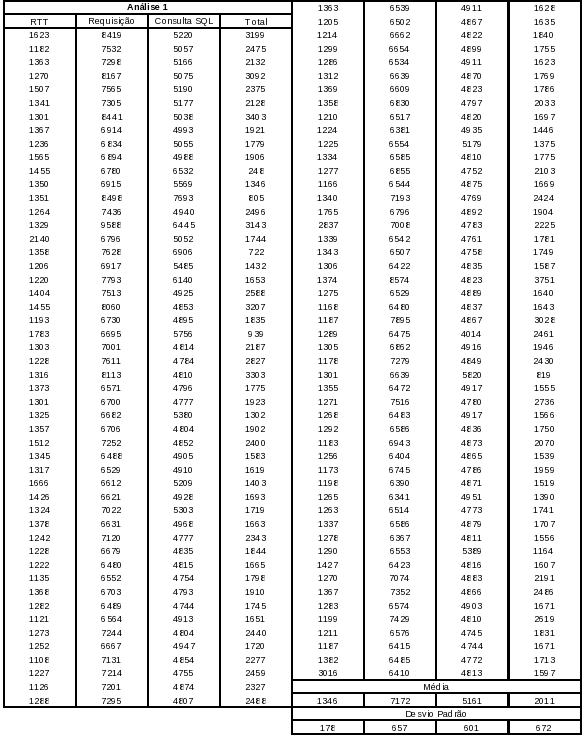
\includegraphics[width=15cm]{analise1.png} 
  \caption{Representação das medições da análise 1.}
  \label{fig:analise1}
\end{figure}

\textbf{Análise 2: }\\
Média do tempo de RTT: \textbf{1293 us}\\
Desvio padrão RTT: \textbf{335 us}\\
Média do tempo total de requisição: \textbf{1932 us}\\
Desvio padrão de requisição: \textbf{909 us}\\
\begin{figure}[htb]
  \centering
  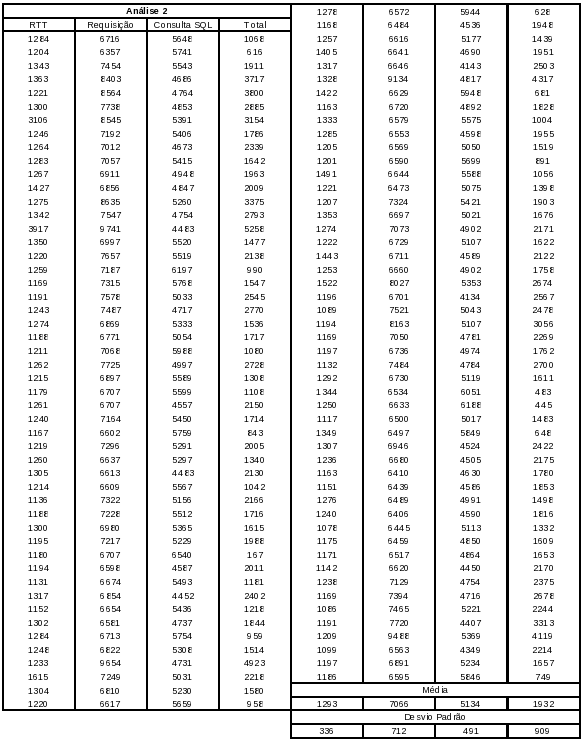
\includegraphics[width=15cm]{analise2.png} 
  \caption{Representação das medições da análise 2.}
  \label{fig:analise2}
\end{figure}

\textbf{Análise 3: }\\
Média do tempo de RTT: \textbf{1355 us}\\
Desvio padrão RTT: \textbf{182 us}\\
Média do tempo total de requisição: \textbf{2043 us}\\
Desvio padrão de requisição: \textbf{864 us}\\
\begin{figure}[htb]
  \centering
  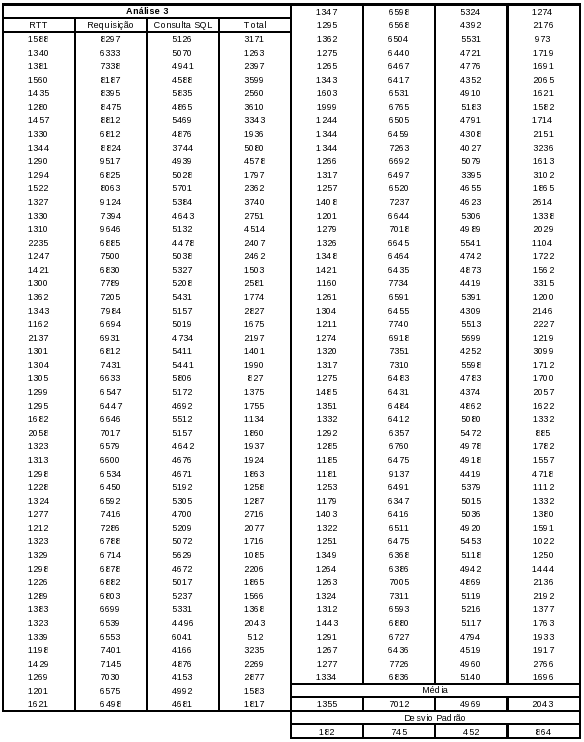
\includegraphics[width=15cm]{analise3.png} 
  \caption{Representação das medições da análise 3.}
  \label{fig:analise3}
\end{figure}

\textbf{Análise 4: }\\
Média do tempo de RTT: \textbf{1424 us}\\
Desvio padrão RTT: \textbf{606 us}\\
Média do tempo total de requisição: \textbf{2065 us}\\
Desvio padrão de requisição: \textbf{868 us}\\
\begin{figure}[htb]
  \centering
  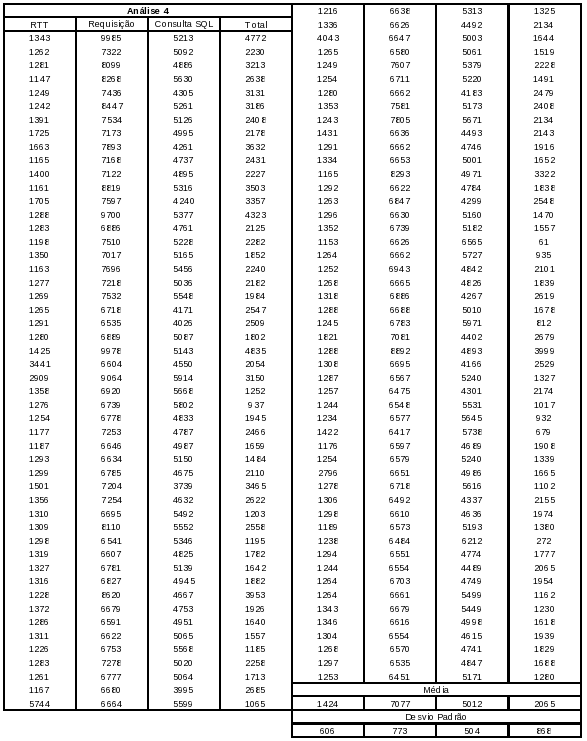
\includegraphics[width=15cm]{analise4.png} 
  \caption{Representação das medições da análise 4.}
  \label{fig:analise4}
\end{figure}

\textbf{Análise 5: }\\
Média do tempo de RTT: \textbf{1338 us}\\
Desvio padrão RTT: \textbf{369 us}\\
Média do tempo total de requisição: \textbf{1974 us}\\
Desvio padrão de requisição: \textbf{846 us}\\
\begin{figure}[htb]
  \centering
  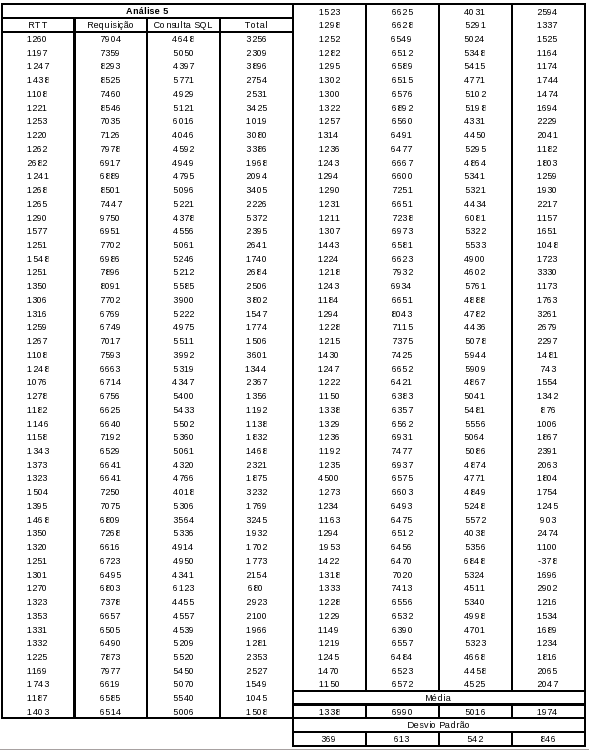
\includegraphics[width=15cm]{analise5.png} 
  \caption{Representação das medições da análise 5.}
  \label{fig:analise5}
\end{figure}

\subsection{Comparação dos projetos feitos em Java RMI e em Sockets TCP em C }
%TODO Fazer a comparação


Pode-se verificar a diferença considerável entre os tempos de RTT para as duas configurações. Obviamente, o tempo para abertura da conexão foi maior para a segunda 
configuração, já que os pacotes devem ser transmitidos através de roteadores e enlaces adicionais, como mostrado no resultado do traceroute acima.\\
De modo a comprovar a influência do tráfego na rede, é visível a grande diferença entre os desvios padrão em porcentagem com relação ao valor absoluto.\\


\section{Confiabilidade e Consistência}
Dois pontos a considerar: robustez quanto à comunicação e consistência dos dados.\\
Tentamos fazer todas as verificações de erros possíveis nas funções das bibliotecas de comunicação com o socket, tanto no lado cliente como no servidor. Ainda assim, não conseguimos implementar um importante caso de exceção: notificar e encerrar o cliente quando o servidor "cai".\\
Com relação à consistência dos dados, esta é garantida pela exclusão mútua nas operações de atualização de avaliação.

\section{Conclusão}
Podemos considerar que a aplicação já está totalmente funcional, todas as consultas estão funcionando corretamente, há a garantia da consistência do banco de dados do cinema e a comunicação entre cliente e servidor está boa, exceto no caso em que o servidor cai, deixando o cliente esperando por uma resposta.\\
Por utilizar o protocolo TCP, a comunicação possui todas as suas vantagens, como confiabilidade na transferência de pacotes, controle de fluxo e controle de congestionamento, o que garante uma qualidade maior à aplicação.\\
A análise de tempo também cumpriu com as espectativas, tendo uma média e um desvio padrão mais baixo para redes próximas e valores mais altos para redes mais distantes.\\
Ao fazer a aplicação em C, o nível de abstração não foi muito alto, pois tivemos que tratar muitos detalhes das conexões.\\
Podemos dizer também que fomos felizes ao utilizar um controle de conexões por threads, pois fica mais fácil de controlar do que com processos, já que quando o processo principal termina, todas as threads também terminam, evitando assim processos zumbi, além de ser mais fácil se implementar exclusão mútua de threads, por exemplo, com semáforos ou mutex lock.\\
Nosso servidor de banco de dados de cinema ainda não é um sistema completo e bem acabado, mas já provê uma base sólida para implementar aplicações gráficas e de maior porte, utilizando o servidor como o núcleo da aplicação. Pretendemos, em versões posteriores, melhorar o programa, resolver bugs e talvez, utilizar uma biblioteca gráfica para tornar sua interface mais usável. 

\section{Código Fonte}

%%%%%%%%%%%%%%%%%%%%%%%%%%%%%%%%%%%%%%%%%%
%%%%%%% add_filme.sh
\subsection{add\_filme.sh}  % 1
\begin{verbatim}
#!/bin/bash

echo "Cadastro de novo filme!"
echo -n "Id: "; read id
echo -n "Titulo: "; read titulo
echo -n "Sinopse: "; read sinopse
echo -n "Sala: "; read sala
echo -n "Horários: "; read horarios

tam_substr=$(echo -n $id\@0000\@000\.00\@$titulo\@$sinopse\@$sala\@
$horarios\@ | wc -c)

# tam_reg deve ser tam_substr + 3~4 (digitos+@)
tam_reg=$(echo -n $tam_substr\@$id\@0000\@000\.00\@$titulo\@$sinopse\@
$sala\@$horarios\@ | wc -c)

# expressão regular ^10*$ casa com qq seq começando com 1 seguida de zeros
if [ $tam_reg = $(echo $tam_reg | grep ^10*$) ]
then
  echo 'Entrou no caso da exceção da virada 10/100/1000'
  tam_reg=$((tam_reg + 1))
else
  echo 'Não entrou na exceção.'
fi

# finalmente, manda os valores para o arquivo
echo -n $tam_reg\@$id\@0000\@000\.00\@$titulo\@$sinopse\@$sala\@
$horarios\@ >> filmes.dat

echo "Registro adicionado com sucesso!"
\end{verbatim}


%%%%%%%%%%%%%%%%%%%%%%%%%%%%%%%%%%%%%%%%%%
%%%%%%% data_access.h
\subsection{data\_access.h} % 2
\begin{verbatim}
#define TAM_MAX_REG 1024 /* 1kB */
#define TAM_MAX_TIT 30
#define TAM_MAX_SIN 900
#define TAM_MAX_SALA 20
#define TAM_MAX_HOR 20

#define TAM_MAX_ATR 900
/* tamanho max dos digitos do tamanho do registro e do id */
#define TAM_REG_ID 20 
/* abc.de (valor de 0 a 100, com 2 dígitos decimais) */
#define TAM_MEDIA 6 
/* cada filme pode ter até 9999 avaliações */
#define TAM_N_AVALIACOES 4 

typedef struct {
  int id;
  char *titulo;
  char *sinopse;
  char *sala;
  char *horarios;
  
  int n_aval; /* número de avaliações */
  float media;

  /* NULL caso seja um único filme ou o último da lista */
  struct filme *prox_filme; 
} filme;

/* 'da' refere-se a data access 
  (para facilitar depois pra chamar as funções) */

/* Função responsável por fazer um parse 
  da string lida do arquivo para um filme */
int da_str_to_filme(filme *f_ret, int *tam_reg, char *f_str);

/* Libera as strings alocadas dinamicamente */
void da_free_strs(filme *f);



/******* Funções a serem chamadas externamente (API) ********/

/* Imprime as informações já formatadas de um filme */
void da_print_full_info(filme *f);

/* Imprime as informações já formatadas de um filme */
void da_print_partial_info(filme *f);

/* Função que retorna um filme a partir de um id */
int da_get_filme_by_id(char *f_str, int id, int *tamanho);

/* Libera toda a memória alocada para o(s) filme(s) (strings e struct) 
 - retorna o numero de filmes desalocados */
int da_free_all(filme *f);

/* Seta uma lista com todos os filmes no arquivo */
int da_get_todos_filmes(filme **filmes);

/* Retorna o número de filmes no arquivo */
int da_get_n_filmes();

/* Retorna uma matriz com os registros todos em formato string pura */
void da_get_raw_strings (char **registros,
   int *tam_registros, int n_registros);

/* Avalia a nota de avaliação do filme e atualiza 
  seu número de atualizações */
int da_avalia_filme(int id, float nota);
\end{verbatim}


%%%%%%%%%%%%%%%%%%%%%%%%%%%%%%%%%%%%%%%%%%
%%%%%%% data_access.c
\subsection{data\_access.c} % 3
\begin{verbatim}
#include <stdio.h>
#include <stdlib.h>
#include "data_access.h"

int da_str_to_filme (filme *f_ret, int *tam_reg, char *f_str) {
  /* Entrada: string crua lida do arquivo, a partir do início de um registro */
  /* Saída: - setup da struct filme passada por referência 
     - tamanho do registro no arquivo
     - valor numérico para erros */
	

  /* Formato do registro no arquivo */
  /* Como há atributos de texto, é difícil manter os registros com 
     tamanho constante no arq */
  /* Assim, uma ideia é usar separadores entre os atributos, assim
     como manter o tamanho do registro */
  /* 
     int tam_total_do_reg (incluindo todos os separadores do registro)
     int id, int avaliacoes, float media [TAMANHO FIXO NO ARQUIVO!], 
     string titulo, string sinopse, 
     string sala, string horarios.
     Separador: @
     Ex: 75@1@0@0@Rei Leão@Sinopse@Kinoplex - sala 10@12h40, 15h, 17h20@
     (contando tudo, incluindo os caracteres de tam_total_do_reg e os separadores)

     Esse esquema do número de caracteres num campo é pra 
     possibilitar a busca entre os registros.
  */

  char str[TAM_MAX_ATR]; /* string fixa bem grande pra comportar qq atributo */

  int i = 0; /* índice de acesso de f_str */
  int j = 0; /* indice para montagem da string  */

  /* tamanho do registro */
  while(f_str[i]!='@') {
    str[j] = f_str[i];
    i++; j++;
  }
  str[j] = '\0';
  *tam_reg = atoi(str);

  /* id */
  i++; j = 0;
  while(f_str[i]!='@') { str[j] = f_str[i]; i++; j++; }
  str[j] = '\0'; 
  f_ret->id = atoi(str);

  /* numero de avaliações */
  i++; j = 0;
  while(f_str[i]!='@') { str[j] = f_str[i]; i++; j++; }
  str[j] = '\0';
  f_ret->n_aval = atoi(str);
	
  /* média */
  i++; j = 0;
  while(f_str[i]!='@') { str[j] = f_str[i]; i++; j++; }
  str[j] = '\0';
  f_ret->media = atof(str);
	
  /* titulo */
  i++; j = 0;
  while(f_str[i]!='@') {
    str[j] = f_str[i];
    i++; j++;
  }
  str[j] = '\0';
  /* aloca a string dinamicamente */
  f_ret->titulo = (char *)malloc((j+1)*sizeof(char));
  sprintf(f_ret->titulo, "%s", str);

  /* Blocos de código similares ao de cima, só que comprimidos  */
  /* sinopse */
  i++; j = 0;
  while(f_str[i]!='@') { str[j] = f_str[i]; i++; j++; } str[j] = '\0';
  f_ret->sinopse = (char *)malloc((j+1)*sizeof(char));
  sprintf(f_ret->sinopse, "%s", str);

  /* sala */
  i++; j = 0;
  while(f_str[i]!='@') { str[j] = f_str[i]; i++; j++; } str[j] = '\0';
  f_ret->sala = (char *) malloc((j+1)*sizeof(char));
  sprintf(f_ret->sala, "%s", str);

  /* horarios */
  i++; j = 0;
  while(f_str[i]!='@' && f_str[i]!='\0') { str[j] = f_str[i]; i++; j++; }
  str[j] = '\0';
  f_ret->horarios = (char *) malloc((j+1)*sizeof(char));
  sprintf(f_ret->horarios, "%s", str);

  /* next - lembra dele? :) */
  f_ret->prox_filme = NULL;

  return(0);
}


void da_print_full_info(filme *f) {
  printf("Id: %d\n", f->id);
  printf("Titulo: %s\n", f->titulo);
  printf("Sinopse: %s\n", f->sinopse);
  printf("Sala: %s\n", f->sala);
  printf("Horários: %s\n", f->horarios);
  printf("Média: %06.2f (%d avaliações)\n", f->media, f->n_aval);
  return;
}

void da_print_partial_info(filme *f) {
  printf("Id: %d\n", f->id);
  printf("Titulo: %s\n", f->titulo);
  return;
}


void da_free_strs(filme *f) {
  free(f->titulo);
  free(f->sinopse);
  free(f->sala);
  free(f->horarios);
  return;
}


int da_free_all(filme *f) {
  /* Esta função desaloca todos os filmes que estiverem na lista, e
     retorna o número desses filmes que foram desalocados.
     A lista precisa ser resolvida de trás pra frente, por isso 
     está sendo usada recursão. */

  int i;

  da_free_strs(f);

  /* Condição de parada (último filme) */
  if(f->prox_filme == NULL) {
    free(f);
    return(0); /* retorna, inicializando contador */
  }

  /* Chamada recursiva */
  i = da_free_all((filme *)f->prox_filme); /* cast pro -Wall n reclamar */

  /* Resolvida a recursão, libera a struct e retorna */
  free(f);
  return(i);

}
	

/* Função a ser chamada pelo SERVIDOR! */
int da_get_filme_by_id(char *f_str, int id, int *tamanho) {

  /* Função responsável por acessar o arquivo dos registros,
     buscar o filme com o id igual ao passado como argumento,
     e retornar o resultado da busca
     Saídas: 0 - filme encontrado (setado em f_str)
     1 - código de retorno que indica que nada foi encontrado
  */

  int tam_reg, id_reg;
  long int cursor = 0; /* indice de leitura do arquivo */
  FILE *arq;

  arq = fopen("filmes.dat", "r");

  while(fscanf(arq, "%d@%d@", &tam_reg, &id_reg) != EOF) {
    /* registro encontrado */
    if(id_reg == id) {
      /* caminha no arquivo até o inicio do registro */
      fseek(arq, cursor, SEEK_SET);
      fgets(f_str, tam_reg, arq);
      *tamanho = tam_reg;
      fclose(arq);
      return(0);
    } else {
      cursor += tam_reg;
      fseek(arq, cursor, SEEK_SET);
    }
  } /* só vai sair do while se não encontrar o filme */
  
  fclose(arq);
  
  return(1);

}


/* Função a ser chamada pelo SERVIDOR! */
int da_get_todos_filmes(filme **filmes_ret) {
  /* Esta função lê o arquivo, instancia uma struct filme para cada registro,
     concatena as structs, e retorna o resultado para o usuário.
     O valor de retorno é um inteiro que representa ou o número de
     registros lidos, ou -1 para erro.
  */

  FILE *arq;
  int tam_reg, i = 0;
  long int cursor = 0; /* indice de leitura do arquivo */
  char buffer[TAM_MAX_REG]; /* 1kB */
  filme *f; /* apontador principal que vai guardar cada um dos registros */

  arq = fopen("filmes.dat", "r");


  /* Enquanto houver registros no arquivo */
  while(fscanf(arq, "%d@", &tam_reg) != EOF) {
    /* Para cada registro, aloca a memória para a struct, seta o registro
     a partir da string lida, seta o cursor do arquivo p/ o próximo */
    i++;
    f = (filme *)malloc(sizeof(filme));
    if(i == 1) {
      /* Início da lista (primeiro registro) */
      *filmes_ret = f;
    }

    fseek(arq, cursor, SEEK_SET); /* pula p/ o inicio do registro */
    fgets(buffer, TAM_MAX_REG, arq); /* lê a string crua no buffer */
    da_str_to_filme(f, &tam_reg, buffer); /* abriga o filme na struct */

    cursor += tam_reg; /* ajuste para a leitura do próximo reg no arq */

    f = (filme *)f->prox_filme; /* atualiza o apontador */
  }

  f = NULL; /* último registro da lista */
  
  fclose(arq);
  
  return(i);
}


/* Retorna o número de filmes no arquivo */
int da_get_n_filmes() {

  FILE *arq;
  int tam_reg, i = 0;
  long int cursor = 0; /* indice de leitura do arquivo */

  arq = fopen("filmes.dat", "r");

  /* Enquanto houver registros no arquivo */
  while(fscanf(arq, "%d@", &tam_reg) != EOF) {
    i++;
    fseek(arq, cursor, SEEK_SET); /* pula p/ o inicio do registro */
    cursor += tam_reg; /* ajuste para a leitura do próximo reg no arq */
  }
  
  fclose(arq);
  
  return(i-1);
	
}

/* Retorna uma matriz com os registros todos em formato string pura */
void da_get_raw_strings (char **registros, int *tam_registros, int n_registros) {
  /* registros já é um vetor de apontadores pra strings, 
     cujo tamanho é o número de registros no arquivo. */
  FILE *arq;
  int tam_reg, i = 0;
  long int cursor = 0; /* indice de leitura do arquivo */

  arq = fopen("filmes.dat", "r");

  /* Enquanto houver registros no arquivo */
  while(fscanf(arq, "%d@", &tam_reg) != EOF) {
    /* Para cada registro, aloca e seta a string */
    registros[i] = (char *)malloc((tam_reg+1) * sizeof(char));
    fseek(arq, cursor, SEEK_SET); /* volta p/ o inicio do registro */
    fgets(registros[i], tam_reg, arq); /* lê a string crua */

    tam_registros[i] = tam_reg; /* seta também os tamanhos dos registros */

    cursor += tam_reg; /* ajuste para a leitura do próximo reg */
		
    i++;
  }
  
  fclose(arq);
  
  return;
}


/* Avalia a nota de avaliação do filme e atualiza seu número de atualizações */
int da_avalia_filme(int id, float nota) {
  /* Retorno
     1 - O filme com o id passado não existe
     0 - Atualização efetuada.
  */

  int tam_reg, id_reg, n_aval;
  float media;
  long int cursor = 0; /* indice de leitura do arquivo */
  FILE *arq;

  /* abre o arquivo com permissão para escrita */
  arq = fopen("filmes.dat", "r+");

  while(fscanf(arq, "%d@%d@%d@%f@", &tam_reg, &id_reg, 
    &n_aval, &media) != EOF) {
    /* registro encontrado */
    if(id_reg == id) {
      /* Cálculo da nova média para o filme */
      float nova_media;
      nova_media = (media*n_aval + nota)/(n_aval+1);
      printf("\n  thread diz: média antiga %06.2f; nova %06.2f\n",
         media, nova_media);
      
      /* caminha no arquivo até o início do número de avaliações */
      fseek(arq, -(2/*@s*/ + TAM_MEDIA + TAM_N_AVALIACOES), SEEK_CUR);

      /* Atualização dos valores: número de avaliações e média */
      fprintf(arq, "%04d@%06.2f@", n_aval+1, nova_media);

      fclose(arq);
      return(0);
    } else {
      cursor += tam_reg;
      fseek(arq, cursor, SEEK_SET);
    }
  } /* só vai sair do while se não encontrar o filme */
  
  fclose(arq);
  
  return(1);

}
\end{verbatim}


%%%%%%%%%%%%%%%%%%%%%%%%%%%%%%%%%%%%%%%%%%
%%%%%%% internet.h
\subsection{internet.h}     % 4
\begin{verbatim}
/*********************************************************************/
/*************************** Cliente *********************************/

/* Função auxiliar que retorna o socketfd da conexão com o servidor */
int client_get_connection(char **argv);

/* Função auxiliar de envio da opção para o servidor */
void client_send_option(int socketfd, char opt);

/* Le o número de filmes passado no próximo parâmetro da stream */
int client_get_n_filmes(int socket);

/* Copia a str de filme da stream */
void client_get_filme_str(int socket, char *f_str);


/*************************** Cliente *********************************/
/*********************************************************************/



/*********************************************************************/
/**************************** Server *********************************/

/* Recebe a opção da stream */
char server_recv_option(int connect_socketfd);

/**************************** Server *********************************/
/*********************************************************************/



/*********************************************************************/
/***************************** Geral *********************************/

/* Envia um caractere para a stream */
void socket_push_char(int socket, char c);

/* Retira um caractere da stream */
char socket_pop_char(int socket);

/* Envia um buffer para a stream */
void socket_push_buffer(int socket, int n, char *buffer);

/* Retira um buffer da stream */
void socket_pop_buffer(int socket, int n, char *buffer);


/***************************** Geral *********************************/
/*********************************************************************/
\end{verbatim}


%%%%%%%%%%%%%%%%%%%%%%%%%%%%%%%%%%%%%%%%%%
%%%%%%% internet.c
\subsection{internet.c}     % 5
\begin{verbatim}
#include "internet.h"
#include "defines.h"
#include "data_access.h"
#include <string.h>
#include <stdio.h>
#include <stdlib.h>
#include <netdb.h>

#include <sys/types.h>
#include <sys/socket.h>
#include <netinet/in.h>
#include <unistd.h>


/*********************************************************************/
/*************************** Cliente *********************************/

/* Função auxiliar que retorna o socketfd da conexão com o servidor */
int client_get_connection(char **argv) {

  int status, socketfd;
  struct addrinfo opcoes;
  struct addrinfo *servinfo;  // will point to the results

  memset(&opcoes, 0, sizeof(opcoes)); // zera a estrutura
  opcoes.ai_family = AF_INET;         // IPv4
  opcoes.ai_socktype = SOCK_STREAM;   // TCP stream sockets
  opcoes.ai_flags = AI_PASSIVE;       // fill in my IP for me

  status = getaddrinfo(argv[1], SERVER_PORT_STR, &opcoes, &servinfo);
  if (status != 0) {
    fprintf(stderr, "getaddrinfo error: %s\n", gai_strerror(status));
    exit(1);
  }

  /* cria o socket com os parâmetros setados */
  socketfd = socket(servinfo->ai_family, servinfo->ai_socktype,
    servinfo->ai_protocol);

  /* faz a conexão com o socket do servidor */
  status = connect(socketfd, servinfo->ai_addr, servinfo->ai_addrlen);

  /* Caso dê algum erro na conexão, pára o cliente */
  if (status == -1){
    fprintf(stderr, "Problema na conexão.\n");
    exit(1);
  }

  freeaddrinfo(servinfo); // libera a estrutura de informações do servidor
  return(socketfd);

}

/* Função auxiliar de envio da opção para o servidor */
void client_send_option(int socketfd, char opt) {
  socket_push_char(socketfd, opt);
  return;
}

/* Le o número de filmes passado no próximo parâmetro da stream */
int client_get_n_filmes(int socket) {

  char str[10], c;
  int i = 0;

	/* Limpa o buffer do canal de comunicação */
  c = socket_pop_char(socket);
	while(c=='\0') c = socket_pop_char(socket);

  /* Preenche uma str com os numeros até chegar o '@' */
  while (c != '@') {
    str[i] = c;
    i++;
    c = socket_pop_char(socket);
  }
  str[i] = '\0';
	
  return(atoi(str));
}

/* Copia a str de filme da stream */
void client_get_filme_str(int socket, char *f_str) {
	
  int i, tam_reg;
  char c, tam_reg_str[TAM_REG_ID];

  /* leitura do tamanho do registro */
  i = 0;
  c = socket_pop_char(socket);
  while (c != '@') {
    //f_str[i] = c;
    tam_reg_str[i] = c;
    i++;
    c = socket_pop_char(socket);
  }
  //f_str[i] = '@';
  tam_reg_str[i] = '\0';

  tam_reg = atoi(tam_reg_str);

  /* Sei o tamanho do registro e sei até onde já li; vou ler o resto */
  tam_reg = tam_reg - i -1; /* numero de caracteres restantes */
  int n = 0;
  char buffer[TAM_MAX_ATR];
  while (n < (tam_reg-1)) {
    n += recv(socket, &buffer[n], (tam_reg - n), 0);
  }
  buffer[n] = '\0';
	
  /* por fim, concatena as strings já lidas, copiando para a str de retorno */
  sprintf(f_str, "%d@%s", (tam_reg+i+1), buffer);
	
  return;
}

/*************************** Cliente *********************************/
/*********************************************************************/


/*********************************************************************/
/**************************** Server *********************************/

/* Recebe a opção da stream */
char server_recv_option(int connect_socketfd) {
  return(socket_pop_char(connect_socketfd));
}


/**************************** Server *********************************/
/*********************************************************************/


/*********************************************************************/
/***************************** Geral *********************************/

/* Envia um caractere para a stream */
void socket_push_char(int socket, char c) {
  int n = 0;
	
  while (n != sizeof(char)) {
    n = send(socket, &c, sizeof(char), 0);
  }

  return;
}

/* Retira um caractere da stream */
char socket_pop_char(int socket) {
  char c;
  int n = 0;

  while (n != sizeof(char)) {
    n = recv(socket, &c, sizeof(char), 0);
  }

  return(c);
}


/* Envia um buffer para a stream */
void socket_push_buffer(int socket, int n, char *buffer) {
  /* 
     Entradas:
     n - número de caracteres a serem escritos;
     buffer - buffer de onde se lê.
  */

  int i = 0;
  
  while(i < (n-1)) {
    i += send(socket, &buffer[i], (n - i), 0);
  }

  return;
}

/* Retira um buffer da stream */
void socket_pop_buffer(int socket, int n, char *buffer) {
  /* 
     Entradas:
     n - número de caracteres a serem lidos;
     buffer - buffer de leitura.
  */

  int i = 0;

  /* Vai acumulando o valor dos bytes já lidos, e enquanto não
   chega ao fim, continua lendo... */
  while(i < (n-1)) {
    i += recv(socket, &buffer[i], (n - i), 0);
  }

  return;
}

/***************************** Geral *********************************/
/*********************************************************************/
\end{verbatim}


%%%%%%%%%%%%%%%%%%%%%%%%%%%%%%%%%%%%%%%%%%
%%%%%%% defines.h
\subsection{defines.h}      % 6 
\begin{verbatim}
#define TRUE 1
#define FALSE 0

#define LISTAR_TODOS_COMPLETO '1'
#define LISTAR_TODOS '2'
#define REG_COMPLETO '3'
#define REG_SINOPSE '4'
#define REG_MEDIA '5'
#define REG_AVALIAR '6'
#define SAIR '7'


// A Porta em que o servidor escuta e na qual os clientes irão se conectar
#define SERVER_PORT 50000
#define SERVER_PORT_STR "50000"

// Tamanho do Buffer de recepcao de mensagens
#define TAM_BUFFER 200

//Tamanho do Buffer de envio de Mensagens
#define TAM_MENSAGEM 200


// Estrutura para definir o atributo a ser passado para a thread
typedef struct {
  int connect_socket;
  int thr_index;
} thread_attr ;
\end{verbatim}


%%%%%%%%%%%%%%%%%%%%%%%%%%%%%%%%%%%%%%%%%%
%%%%%%% server.c
\subsection{server.c}       % 7
\begin{verbatim}
// Bibliotecas comuns
#include <string.h>
#include <stdio.h>
#include <stdlib.h>
#include <netdb.h>
#include "defines.h"
#include "internet.h"
#include "data_access.h"
#include <signal.h>

// Biblioteca para threads
#include <pthread.h>

// Exclusão Mútua
#include <semaphore.h>

// Bibliotecas para manipulacao de sockets
#include <sys/types.h>
#include <sys/socket.h>
#include <netinet/in.h>
#include <unistd.h>

// número máximo de possíveis conexões pendentes na fila
#define QTDE_CONEXOES 10 
/* valor maximo de threads simultaneas */
#define PTHREAD_THREADS_MAX 10  


/* Variável global que armazena o status para cada thread
   TRUE: significa que ela está disponível;
   FALSE: significa que ela não está disponível.
*/
int available_thrs[QTDE_CONEXOES];


/* Semáforo global usado para garantir exclusão mútua entre as threads 
   no uso do arquivo (escrita). */
sem_t semaphore;


/**************************************************************/
/******[inicio] Funções que implementam os casos de uso  ******/

/* ## 1 ## */
void server_lista_todos_completo(int socket) {

  /*
    Esta função envia ao cliente uma sequencia de caracteres no formato:
    n_filmes@str_filme1@str_filme2@...@
  */

  /* Envio do numero de filmes */
  int n_filmes, n, i;
  char n_filmes_str[10]; /* max: 999999999@ */

  n_filmes = da_get_n_filmes();
  sprintf(n_filmes_str, "%d@", n_filmes);

  n = 0;
  while (n < strlen(n_filmes_str)) {
    n = send(socket, n_filmes_str, strlen(n_filmes_str), 0);
  }

  /* Agora, para cada filme, envia sua string crua. */
  char **registros;
  int *tam_reg;
  registros = (char **)malloc(n_filmes*sizeof(char *));
  tam_reg = (int *)malloc(n_filmes*sizeof(int));
  da_get_raw_strings(registros, tam_reg, n_filmes);

  for (i = 0; i < n_filmes; i++) {
    n = 0;
    socket_push_buffer(socket, tam_reg[i], registros[i]);
    free(registros[i]);
  }
  free(registros);
  free(tam_reg);

  return;
}

/* ## 2 ## */
void server_lista_todos(int socket) {
  /* O servidor faz exatamente a mesma coisa para a 
   listagem parcial. Todas informações são passadas
   para o cliente, mas este só imprime algumas delas. */
  server_lista_todos_completo(socket);
  return;
}

/* ## 3 ## */
void server_reg_completo(int socket) {
  
  /* servidor lê o ID que está sendo passado */
  char c, id_procurado[TAM_REG_ID]; /* 20 */
  int i = 0, tam_reg;

  /* leitura do ID pesquisado pelo cliente */
  c = socket_pop_char(socket);
  while (c!='@') {
    id_procurado[i] = c;
    c = socket_pop_char(socket);
    i++;
  }
  id_procurado[i] = '\0';

  int id;
  id = atoi(id_procurado);

  printf("  id requisitado: %d\n", id);

  /* Função que faz a busca.
     Retorna 1 se n encontrou nenhum filme.
     Caso contrário, aloca a memória e seta o filme. */
  
  char f_str[TAM_MAX_REG];

  /* se não encontrou nenhum filme, envia erro ao cliente */
  if (da_get_filme_by_id(f_str, id, &tam_reg) == 1) {
    socket_push_char(socket, '#');
    return;
  }

  /* se encontrou... */
  /* envia caractere de confirmação */
  socket_push_char(socket, '%');
  
  /* envia o filme */
  socket_push_buffer(socket, tam_reg, f_str);

  return;
}

/* ## 4 ## */
void server_reg_sinopse(int socket) {
  /* Neste caso, o servidor faz exatamente o mesmo  
   * que na listagem completa de um registro:
   * 1- Recebe o registro procurado;
   * 2- Faz a busca;
   * 3- Se não encontrar o filme, retorna o caractere '#'
   * 4- Se encontrar, retorna a string crua do filme
   */
  server_reg_completo(socket);
  return;
}

/* ## 5 ## */
void server_reg_media(int socket) {
  /* Neste caso, o servidor faz exatamente o mesmo  
   * que na listagem completa de um registro:
   * 1- Recebe o registro procurado;
   * 2- Faz a busca;
   * 3- Se não encontrar o filme, retorna o caractere '#'
   * 4- Se encontrar, retorna a string crua do filme
   */
  server_reg_completo(socket);
  return;
}

/* ## 6 ## */
void server_reg_avalia(int socket) {

  /* servidor lê o ID que está sendo passado */
  char c, id_avaliar[TAM_REG_ID] /*20*/, nota_s[7];
  int i = 0;

  /* leitura do ID requisitado pelo cliente p/ avaliação */
  do { 
    c = socket_pop_char(socket);
  } while (c=='\0'); /* limpa stream */
  while (c!='@') {
    id_avaliar[i] = c;
    c = socket_pop_char(socket);
    i++;
  }
  id_avaliar[i] = '\0';

  int id;
  id = atoi(id_avaliar);

  /* leitura da nota */
  i = 0;
  do { 
    c = socket_pop_char(socket);
  } while (c=='\0'); /* limpa stream */
  while (c!='@') {
    nota_s[i] = c;
    c = socket_pop_char(socket);
    i++;
  }
  nota_s[i] = '\0';

  float nota;
  nota = atof(nota_s);

  printf("  id p/ avaliar: %d\n", id);

  printf("  nota enviada: %06.2f", nota);

  /* 
   * Importante: Uso do semáforo para controle de concorrência
   * do recurso (no caso o arquivo), garantido exclusão mútua,
   * isto é, apenas uma thread poderá escrever nele por vez.
   */
  sem_wait(&semaphore); /* trava até o semáforo estar liberado */

  /**************************************/
  /* [Início] Região com Exclusão Mútua */
  int status;
  /* sleep(10); */ /* testes */
  
  /*
   * Função que realiza a avaliação:
   * Retorna 1 se o filme não existe.
   * Retorna 0 se ocorreu tudo bem.
   */
  status = da_avalia_filme(id, nota);
  /** [Fim] Região com Exclusão Mútua ***/
  /**************************************/

  sem_post(&semaphore); /* libera o semáforo */

  /* se não encontrou nenhum filme, envia erro ao cliente */
  if (status == 1) {
    socket_push_char(socket, '#');
  } else {
    /* se encontrou, envia caractere de confirmação */
    socket_push_char(socket, '%');
  }

  return;
}

/*******[fim] Funções que implementam os casos de uso  ********/
/**************************************************************/


/* Implementa o comportamento de cada thread */
void *trata_conexao (void *a) {
  
  int connect_socketfd;
  int t;

  char option;

  /* cast pra dizer que é um ap pra thread_attr */
  connect_socketfd = ((thread_attr *)a)->connect_socket;
  t = ((thread_attr *)a)->thr_index;

  /* recebe a opção enviada pelo cliente. */
  option = server_recv_option(connect_socketfd);
	
  printf("opção enviada pelo cliente: %c\n", option);

  /* Verificação do caso de saída e chamadas para cada caso específico */
  while(option != SAIR) {
      
    switch(option) {
			
    case LISTAR_TODOS_COMPLETO:
      server_lista_todos_completo(connect_socketfd);
      break;
    case LISTAR_TODOS:
      server_lista_todos(connect_socketfd);
      break;
    case REG_COMPLETO:
      server_reg_completo(connect_socketfd);
      break;
    case REG_SINOPSE:
      server_reg_sinopse(connect_socketfd);
      break;
    case REG_MEDIA:
      server_reg_media(connect_socketfd);
      break;
    case REG_AVALIAR:
      server_reg_avalia(connect_socketfd);
      break;
    }

    /* recebe a opção enviada pelo cliente. */
    option = server_recv_option(connect_socketfd);
    printf("opção enviada pelo cliente: %c\n", option);
  }
	
  printf("Thread %d diz: terminei! Fechando o socket %d...\n",
    t, connect_socketfd);
  close(connect_socketfd);

  /* thread seta o valor do vetor de disponíveis para TRUE novamente */
  available_thrs[t] = TRUE;

  pthread_exit(NULL);
}

//Trata o sinal de interrupcao mandar uma mensagem antes de encerrar
void trata_SIGINT(int sig) {
  printf("\nEncerrando o servidor...\n");
  /* Mesmo usando o socket de listen como variável global, e dando
     um close(list_socket) aqui, continua com o problema do bind
     depois de interromper o servidor. Isso acontece por causa da
     implementação do TCP no Kernel, que demora algum tempo pra
     liberar novamente a porta para bind. */

  /* Desaloca recursos para o semáforo */
  sem_destroy(&semaphore);

  exit(0);
}

int main() {

  // Sockets de escuta e de conexao
  int listen_socketfd, connect_socketfd; 

  signal(SIGINT,trata_SIGINT);

  int status;
  struct addrinfo opcoes;
  struct addrinfo *servinfo;  // Informações do meu endereço

  memset(&opcoes, 0, sizeof(opcoes)); // zera a estrutura
  opcoes.ai_family = AF_INET;         // IPv4
  opcoes.ai_socktype = SOCK_STREAM;   // TCP
  opcoes.ai_flags = AI_PASSIVE;       // fill in my IP for me

  status = getaddrinfo(NULL, SERVER_PORT_STR, &opcoes, &servinfo);
  if (status != 0) {
    fprintf(stderr, "getaddrinfo error: %s\n", gai_strerror(status));
    exit(1);
  }

  // cria o socket TCP de escuta
  listen_socketfd = socket(servinfo->ai_family,
    servinfo->ai_socktype, servinfo->ai_protocol);
  printf("Socket TCP de escuta criado!\n");
  
  //Atribui a porta utilizada ao socket de escuta
  status = bind(listen_socketfd, servinfo->ai_addr,
    servinfo->ai_addrlen); 
  if (status == -1) {
    fprintf(stderr, "error on binding the socket to a port\n");
    exit(1);
  }
  freeaddrinfo(servinfo); // libera a estrutura de informações do servidor

  /* Atribui o socket como ouvinte das conexões. */
  listen(listen_socketfd, QTDE_CONEXOES);

  /* Inicializa o semáforo. O número de recursos compartilhados 
     é 1 (apenas uma thread pode usar o arquivo para escrita de
     cada vez) - este é o terceiro argumento. O segundo argumento
     é uma flag com valor padrão 0. */
  sem_init(&semaphore, 0, 1);


  /* Threads Time! */
  //  pthread_t thread;
  pthread_t threads[QTDE_CONEXOES];
  int i, t;

  /* Inicializa o vetor de threds disponíveis */
  for (i = 0; i < QTDE_CONEXOES; i++) available_thrs[i] = TRUE;

  struct sockaddr_storage client_addr;
  socklen_t addr_size;

  while(TRUE) {
    /* Aceitação da conexão. */
    printf("Esperando alguma conexao...\n");
    connect_socketfd = accept(listen_socketfd,
      (struct sockaddr *)&client_addr, &addr_size);
    if (connect_socketfd == -1){
      printf("Problema na conexão.\n");
      continue; /* Desiste dessa conexão. */
    }
    printf("Conexao aceita!\n");
    
    /* Seleciona a primeira thread disponível */
    /* t recebe o indice da primeira thread disponível */
    t = -1;
    for (i = 0; i < QTDE_CONEXOES; i++) {
      if (available_thrs[i]==TRUE) {
	t = i; break;
      }
    }
    
    /* caso não haja nenhuma thread disponível, fecha a conexão e volta a ouvir */
    if (t == -1) { 
      printf("Não há thread disponível para aceitar a conexão.\n");
      close(connect_socketfd); continue;
    }

    /* Inicia a thread e passa o connect_socketfd pra ela. */
    available_thrs[t] = FALSE; /* agora essa thread não está disponível */
    printf("Main diz: vou passar para a thread o socket %d.\n", connect_socketfd);
    /* inicializa o atributo a passar para a thread */
    thread_attr a;
    a.connect_socket = connect_socketfd;
    a.thr_index = t;
    pthread_create(&threads[t], NULL, trata_conexao, (void *)&a);

  }

  return(0);
}
\end{verbatim}


%%%%%%%%%%%%%%%%%%%%%%%%%%%%%%%%%%%%%%%%%%
%%%%%%% client.c
\subsection{client.c}       % 8
\begin{verbatim}
//Bibliotecas comuns
#include <string.h>
#include <stdio.h>
#include <stdlib.h>
#include <netdb.h>   //Para usar o gethostbyname
#include "data_access.h"
#include "defines.h"
#include "internet.h"

//Bibliotecas para manipulacao de sockets
#include <sys/types.h>
#include <sys/socket.h>
#include <netinet/in.h>
#include <unistd.h>


/* Função auxiliar para tratamento de entrada */
char read_option() {
  /* considera os possiveis erros e só sai quando o usuario
     digitar um caractere válido */

  char c, aux;

  while(TRUE) {

    /* Mensagem com as opções... */
    system("clear");
    printf("Escolha uma entre as opções e tecle Enter:\n");
    printf("(opções com (*) requererão o id do filme)\n");
    printf(" [1] Listar todas as informações de todos os filmes.\n");
    printf(" [2] Listar id e título de todos os filmes.\n");
    printf(" [3] Listar todas as informações de um filme. (*)\n");
    printf(" [4] Mostrar a sinopse de um filme. (*)\n");
    printf(" [5] Mostrar a avaliação de um filme. (*)\n");
    printf(" [6] Avaliar um filme! (*)\n");
    printf(" [7] Sair\n  ");

    c = getchar(); aux = getchar();
    if((c==SAIR || c==LISTAR_TODOS_COMPLETO || c==LISTAR_TODOS ||
	c==REG_COMPLETO || c==REG_SINOPSE || c==REG_MEDIA ||
	c==REG_AVALIAR) && aux=='\n') {
      /* se a opcao lida é válida e o próximo caractere foi Enter, 
	 retorna o caractere válido digitado*/
      return(c);
    } else {
      /* caso contrário, 'come' todo o resto da linha e volta às msgs */
      if(aux != '\n') { while(getchar()!='\n'); }
    }
  } /* fim do while */

}



/**************************************************************/
/******[inicio] Funções que implementam os casos de uso  ******/

/* ## 1 ## */
void client_lista_todos_completo(int socketfd) {
  /* 
     Não é necessário enviar mais informações ao servidor, apenas
     aguardar um retorno.
     O formato desse retorno será:
     n_filmes@str_do_filme1@str_do_filme2@str_do_filme3@
  */

  int n_filmes, i;
  char filme_str[TAM_MAX_REG]; /* 1024 */
  filme *lista_filmes, *f, *last_f;
	
  /* Leitura do número de filmes retornado pelo servidor */
  n_filmes = client_get_n_filmes(socketfd);

  if (n_filmes == 0) {
    printf("Não há filmes no servidor!\n");
    printf("Tecle Enter para continuar...");
    getchar();
    return;
  }
  printf("Número de filmes encontrados: %d\n\n", n_filmes);

  for (i = 0; i < n_filmes; i++) {

    int tam_filme;
		
    /* Le a string do filme */
    client_get_filme_str(socketfd, filme_str);

    /* Aloca a estrutura para guardar o filme */
    f = (filme *)malloc(sizeof(filme));
    da_str_to_filme(f, &tam_filme, filme_str);

    /* Seta a lista dos filmes */
    if (i==0){ /* primeiro filme */
      lista_filmes = f;
    }
    else {
      last_f->prox_filme = f; /* concatena o filme à lista */
    }
    last_f = f; /* atualiza o apontador para o último filme */
  }
	
  /* para cada filme na lista, chama da_print_full_info(f) */
  for (f = lista_filmes; f != NULL; f = (filme *)f->prox_filme) {
    da_print_full_info(f);
    printf("\n-------------------------\n");
  }
	
  /* libera a memória dos filmes */
  da_free_all(lista_filmes);

  printf("Tecle Enter para continuar...");
  getchar();

  return;
}

/* ## 2 ## */
void client_lista_todos(int socketfd) {

  /* Cliente praticamente igual para a listagem completa. */
  int n_filmes, i;
  char filme_str[TAM_MAX_REG]; /* 1024 */
  filme *lista_filmes, *f, *last_f;
	
  n_filmes = client_get_n_filmes(socketfd);

  if (n_filmes == 0) { printf("Não há filmes no servidor!\n");
    printf("Tecle Enter para continuar..."); getchar(); return;
  }
  printf("Número de filmes encontrados: %d\n\n", n_filmes);

  for (i = 0; i < n_filmes; i++) {

    int tam_filme;
    client_get_filme_str(socketfd, filme_str);
    f = (filme *)malloc(sizeof(filme));
    da_str_to_filme(f, &tam_filme, filme_str);
    if (i==0) { lista_filmes = f;} else { last_f->prox_filme = f; }
    last_f = f; /* atualiza o apontador para o último filme */
  }
	
  /* para cada filme na lista, chama da_print_partial_info(f) */
  for (f = lista_filmes; f != NULL; f = (filme *)f->prox_filme) {
    da_print_partial_info(f);
    printf("\n-------------------------\n");
  }
	
  da_free_all(lista_filmes);
  printf("Tecle Enter para continuar..."); getchar();
  return;
}

/* ## 3 ## */
void client_reg_completo(int socketfd) {

  char c, id_procurado[TAM_REG_ID]; /* 20 */
  int i = 0;

  /* Leitura do id procurado (digito p/ dig.) */
  printf("ID do filme: ");
  c = getchar();
  while (c!='\n') { id_procurado[i] = c; i++; c = getchar(); }
  id_procurado[i] = '@'; /* coloca um @ para finalizar o id */

  /* envia o id procurado ao servidor */
  socket_push_buffer(socketfd, i+1, id_procurado);

  /* leitura da resposta do servidor */
  do {
    c = socket_pop_char(socketfd);
  } while(c == '\0'); /* limpa a stream */
  
  /* Caso não tenha encontrado nenhum filme */
  if (c == '#') {
    printf("\nFilme não encontrado.\n");
  } else {
    /* recebe a str do filme encontrado */
    char f_str[TAM_MAX_REG];
    i = 0;
    c = socket_pop_char(socketfd);
    while(c != '\0') { 
      f_str[i] = c;
      c = socket_pop_char(socketfd);
      i++;
    }

    /* monta a estrutura de filme */
    filme f;
    int tam_reg;
    da_str_to_filme(&f, &tam_reg, f_str);

    /* Imprime resultado da pesquisa */
    printf("Filme encontrado!\n\n");
    da_print_full_info(&f);
  }

  printf("\nAperte Enter para continuar...");
  getchar();

  return;
}

/* ## 4 ## */
void client_reg_sinopse(int socketfd) {

  /* Cópia do caso de uso para a listagem completa de um filme, 
     diferenciando apenas a impressão dos dados.*/
  
  char c, id_procurado[TAM_REG_ID]; int i = 0;

  printf("ID do filme: "); c = getchar();
  while (c!='\n') { id_procurado[i] = c; i++; c = getchar(); }
  id_procurado[i] = '@'; /* coloca um @ para finalizar o id */

  socket_push_buffer(socketfd, i+1, id_procurado);

  do { c = socket_pop_char(socketfd);
  } while(c == '\0'); /* limpa a stream */
  
  if (c == '#') { printf("\nFilme não encontrado.\n"); }
  else {
    char f_str[TAM_MAX_REG];
    i = 0; c = socket_pop_char(socketfd);
    while(c != '\0') { 
      f_str[i] = c; 
      c = socket_pop_char(socketfd);
      i++;
    }

    filme f; int tam_reg;
    da_str_to_filme(&f, &tam_reg, f_str);

    printf("Filme encontrado!\n\n");
    printf("Sinopse: %s\n", f.sinopse);
  }

  printf("\nAperte Enter para continuar...");
  getchar();

  return;
}

/* ## 5 ## */
void client_reg_media(int socketfd) {

  /* Cópia do caso de uso para a listagem completa de um filme, 
     diferenciando apenas a impressão dos dados.*/

  char c, id_procurado[TAM_REG_ID]; int i = 0;

  printf("ID do filme: "); c = getchar();
  while (c!='\n') { id_procurado[i] = c; i++; c = getchar(); }
  id_procurado[i] = '@'; /* coloca um @ para finalizar o id */

  socket_push_buffer(socketfd, i+1, id_procurado);

  do { c = socket_pop_char(socketfd);
  } while(c == '\0'); /* limpa a stream */
  
  if (c == '#') { printf("\nFilme não encontrado.\n"); }
  else {
    char f_str[TAM_MAX_REG];
    i = 0; c = socket_pop_char(socketfd);
    while(c != '\0') { 
      f_str[i] = c; 
      c = socket_pop_char(socketfd);
      i++;
    }

    filme f; int tam_reg;
    da_str_to_filme(&f, &tam_reg, f_str);

    printf("Filme encontrado!\n\n");
    printf("Média: %3.2f (%d avaliações)\n", f.media, f.n_aval);
  }

  printf("\nAperte Enter para continuar...");
  getchar();

  return;
}

/* ## 6 ## */
void client_reg_avalia(int socketfd) {

  char c, id_avaliar[TAM_REG_ID] /*20*/, nota[7];
  int i, j;

  /* Leitura do id do filme para avaliar e nota */
  printf("ID do filme a avaliar: ");
  i = 0; c = getchar();
  while (c!='\n') { id_avaliar[i] = c; i++; c = getchar(); }
  id_avaliar[i] = '@'; /* coloca um @ para finalizar o id */
  printf("Nota [formato: abc.de]: ");
  j = 0; c = getchar();
  while (c!='\n') { nota[j] = c; j++; c = getchar(); }
  nota[j] = '@'; /* coloca um @ para finalizar a nota*/

  /* envia o id e a nota ao servidor */
  socket_push_buffer(socketfd, i+1, id_avaliar);
  socket_push_buffer(socketfd, j+1, nota);

  /* leitura da resposta do servidor */
  do {
    c = socket_pop_char(socketfd);
  } while(c == '\0'); /* limpa a stream */
  
  /* Caso não tenha encontrado nenhum filme */
  if (c == '#') {
    printf("\nFilme não encontrado.\n");
  } else {
    printf("\nAvaliação realizada com sucesso!\n");
  }

  printf("\nAperte Enter para continuar...");
  getchar();

  return;
}

/*******[fim] Funções que implementam os casos de uso  ********/
/**************************************************************/



int main(int argc, char** argv) {

  /* Caso não haja o nome do servidor, da um erro */
  if (argc != 2) {
    fprintf(stderr, "uso: ./client <nome do servidor>\n");
    exit(1);
  }
	
  /* Estabelece a conexão com o servidor */
  int socketfd; //Socket de conexao
  socketfd = client_get_connection(argv);

  /* Loop da interface e chamadas para as funções que implementam cada 
     uso do sistema. */
  char c;
		
  c = read_option();
    
  /* Envia a opção escolhida ao servidor (mesmo se for Sair) */
  client_send_option(socketfd, c);

  while(c != SAIR) {
      
    switch(c) {
	
    case LISTAR_TODOS_COMPLETO:
      client_lista_todos_completo(socketfd);
      break;
    case LISTAR_TODOS:
      client_lista_todos(socketfd);
      break;
    case REG_COMPLETO:
      client_reg_completo(socketfd);
      break;
    case REG_SINOPSE:
      client_reg_sinopse(socketfd);
      break;
    case REG_MEDIA:
      client_reg_media(socketfd);
      break;
    case REG_AVALIAR:
      client_reg_avalia(socketfd);
      break;
			
    }
    
    c = read_option();
    client_send_option(socketfd, c);

  }
	
  close(socketfd); // fecha a conexão com o servidor
  return(0);

}
\end{verbatim}


%%%%%%%%%%%%%%%%%%%%%%%%%%%%%%%%%%%%%%%%%%
%%%%%%% Makefile
\subsection{Makefile}       % 9 
\begin{verbatim}
# Variáveis
CC = gcc
CC_FLAGS = -ggdb -Wall


# Dependências gerais
all: client server relatorio

# Cliente
client: data_access.o internet.o client.o
  $(CC) $(CC_FLAGS) data_access.o internet.o client.o -o client

client.o: client.c data_access.h internet.h defines.h
  $(CC) $(CC_FLAGS) -c client.c

# Servidor
server: data_access.o internet.o server.o
  $(CC) $(CC_FLAGS) -pthread data_access.o internet.o server.o -o server

server.o: server.c data_access.h internet.h defines.h
  $(CC) $(CC_FLAGS) -pthread -c server.c

# Bibliotecas
data_access.o: data_access.c data_access.h defines.h
  $(CC) $(CC_FLAGS) -c data_access.c

internet.o: internet.c internet.h defines.h
  $(CC) $(CC_FLAGS) -c internet.c


# Relatório (LaTeX)
relatorio:
  pdflatex relatorio.tex

# Clean
clean:
  rm *.o client server
  rm *.aux *.toc *.pdf *.log
\end{verbatim}

\section{Anexo}
%\begin{figure}[htb]
%  \centering
%  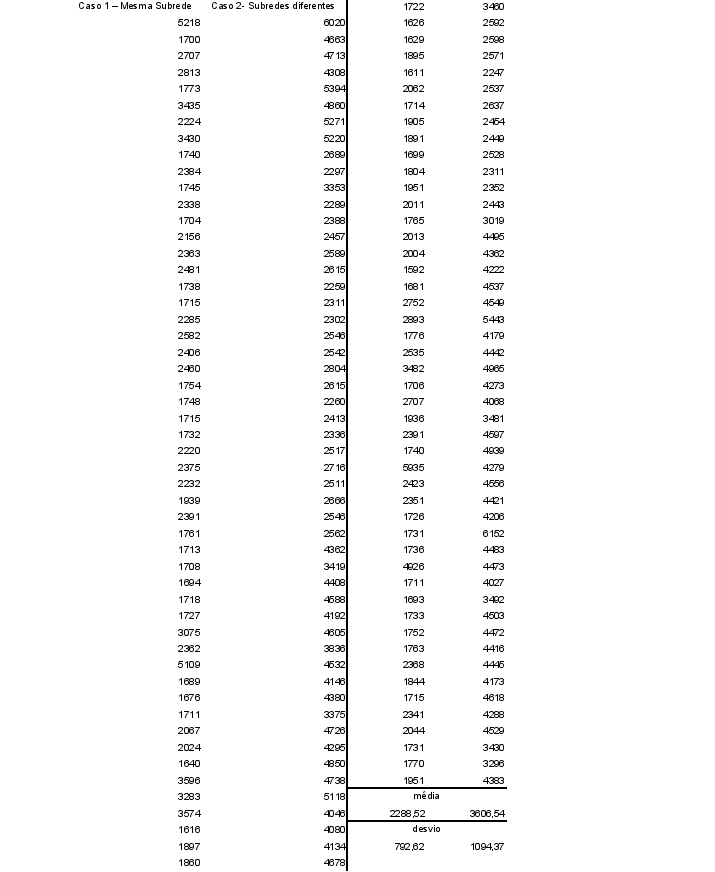
\includegraphics[width=15cm]{medicoes.png} 
%  \caption{Representação das medições para a consulta.}
%  \label{fig:rtt}
%\end{figure}

\begin{thebibliography}{99}
\bibitem{R1} HALL, Brian. Beej's Guide to Network Programming. Disponível em: http://http://beej.us/guide/bgnet/output/html/multipage/index.html.
\end{thebibliography}

\end{document}
